\begin{figure}[t]
    \centering
    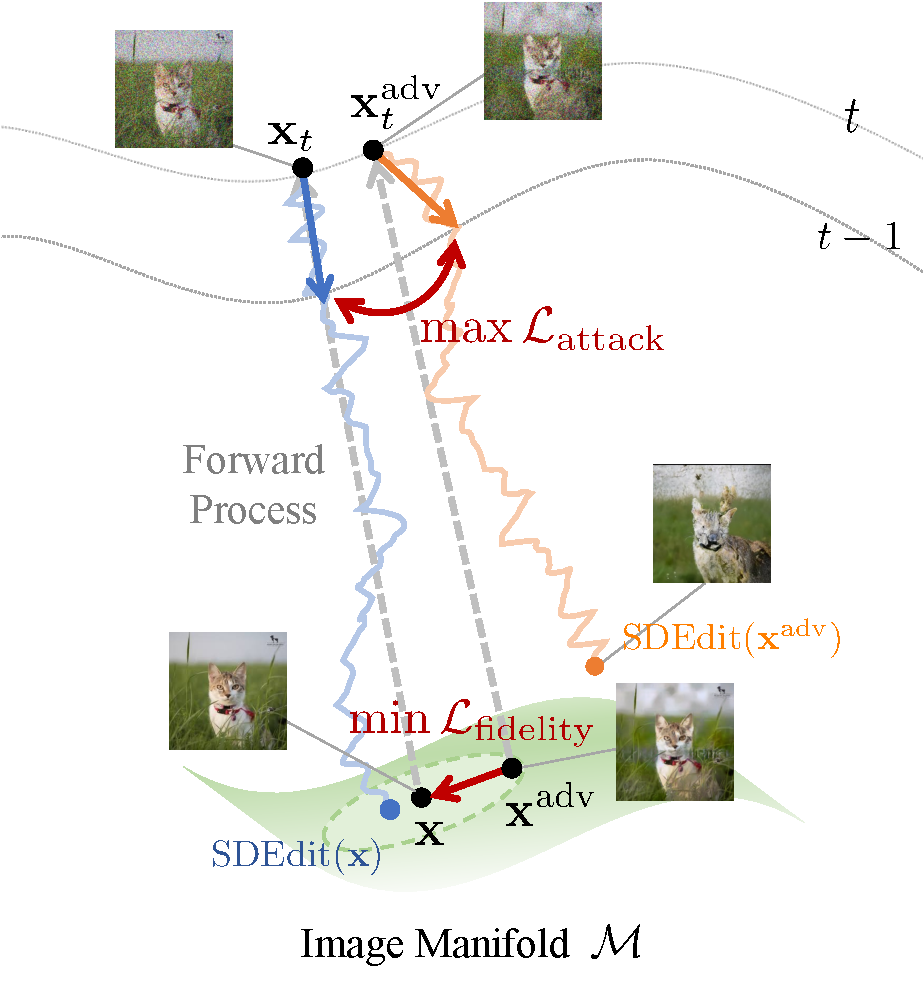
\includegraphics[width=1\linewidth]{figures/manifold.pdf}
    \caption{Conceptual illustration of our method. We randomly forward both the clean image $\mathbf{x}$ and adversarial image $\mathbf{x}^{\adv}$ to noise level $t$, then utilize our feature attacking loss to maximize the feature distance between noisy latent $\mathbf{x}_t$ and $\mathbf{x}^{\adv}_t$ in the reverse process of diffusion models while imposing our fidelity loss as a constraint to ensure the adversarial image from being deviated from the original image. We update the $\mathbf{x}^{\adv}$ in latent space instead of in pixel space to ensure the naturalness of $\mathbf{x}^{\adv}$.}
    \label{concept}
\end{figure}


\section{Methodology}

\subsection{Threat Model and Problem Setting}
The malicious user collects an image $\mathbf{x}$ from the internet and uses SDEdit \cite{meng2021sdedit} to generate unauthorized image translations or editing, denoted as $\text{SDEdit}(\mathbf{x}, t)$, that manipulates the original input image $\mathbf{x}$.

Our work aims to safeguard the input image $\mathbf{x}$ from the authorized manipulations by crafting an adversarial image $\mathbf{x}^{\adv}$ by adding imperceptible perturbation to disrupt the reverse diffusion process of SDEdit for corrupted editions.

For example, we want the main object of the image, e.g., the cat in the source image $\mathbf{x}$ as shown in Figure~\ref{concept} unable to be reconstructed by the reverse diffusion process. Meanwhile, the adversarial image should maintain similarity to the source image to ensure fidelity. The reason why we target SDEdit as our threat model is that it is recognized as the most common and general operation in diffusion-based unconditional image translations and conditional image editing. Additionally, it has been incorporated into various editing pipelines~\cite{tsaban2023leditsrealimageediting, zhang2023inversion}. Here we focus on the unconditional image translations for our main study, as they are essential in both unconditional and conditional editing pipelines. Formally, our objective to effectively safeguard images while maintaining fidelity is formulated as:

\begin{equation}
    \begin{aligned}
        & \max_{\mathbf{x}^{\adv} \in \mathcal{M}} d(\text{SDEdit}(\mathbf{x}, t), \text{SDEdit}(\mathbf{x}^{\adv}, t)) \\
    & \text{subject to } d^{\prime}(\mathbf{x}, \mathbf{x}^{\adv}) \leq \delta,
    \end{aligned}
    \label{eq:probelm_setting_constraint}
\end{equation}

where $\mathcal{M}$ indicates natural image manifold, $d$, $d^{\prime}$ indicate image distance functions and $\epsilon$ denotes the fidelity budget.

In the following sections, we first present a conceptual illustration of our method, followed by our framework for solving the optimization problem. We then discuss the novel design of our attacking loss and fidelity constraints, which provide more efficient criteria compared to previous methods for solving the image protection optimization problem using PGD. Finally, we introduce an advanced design to enhance image protection quality by latent optimization via victim-model-agnostic VAE.

\begin{figure*}[t]
    \centering
    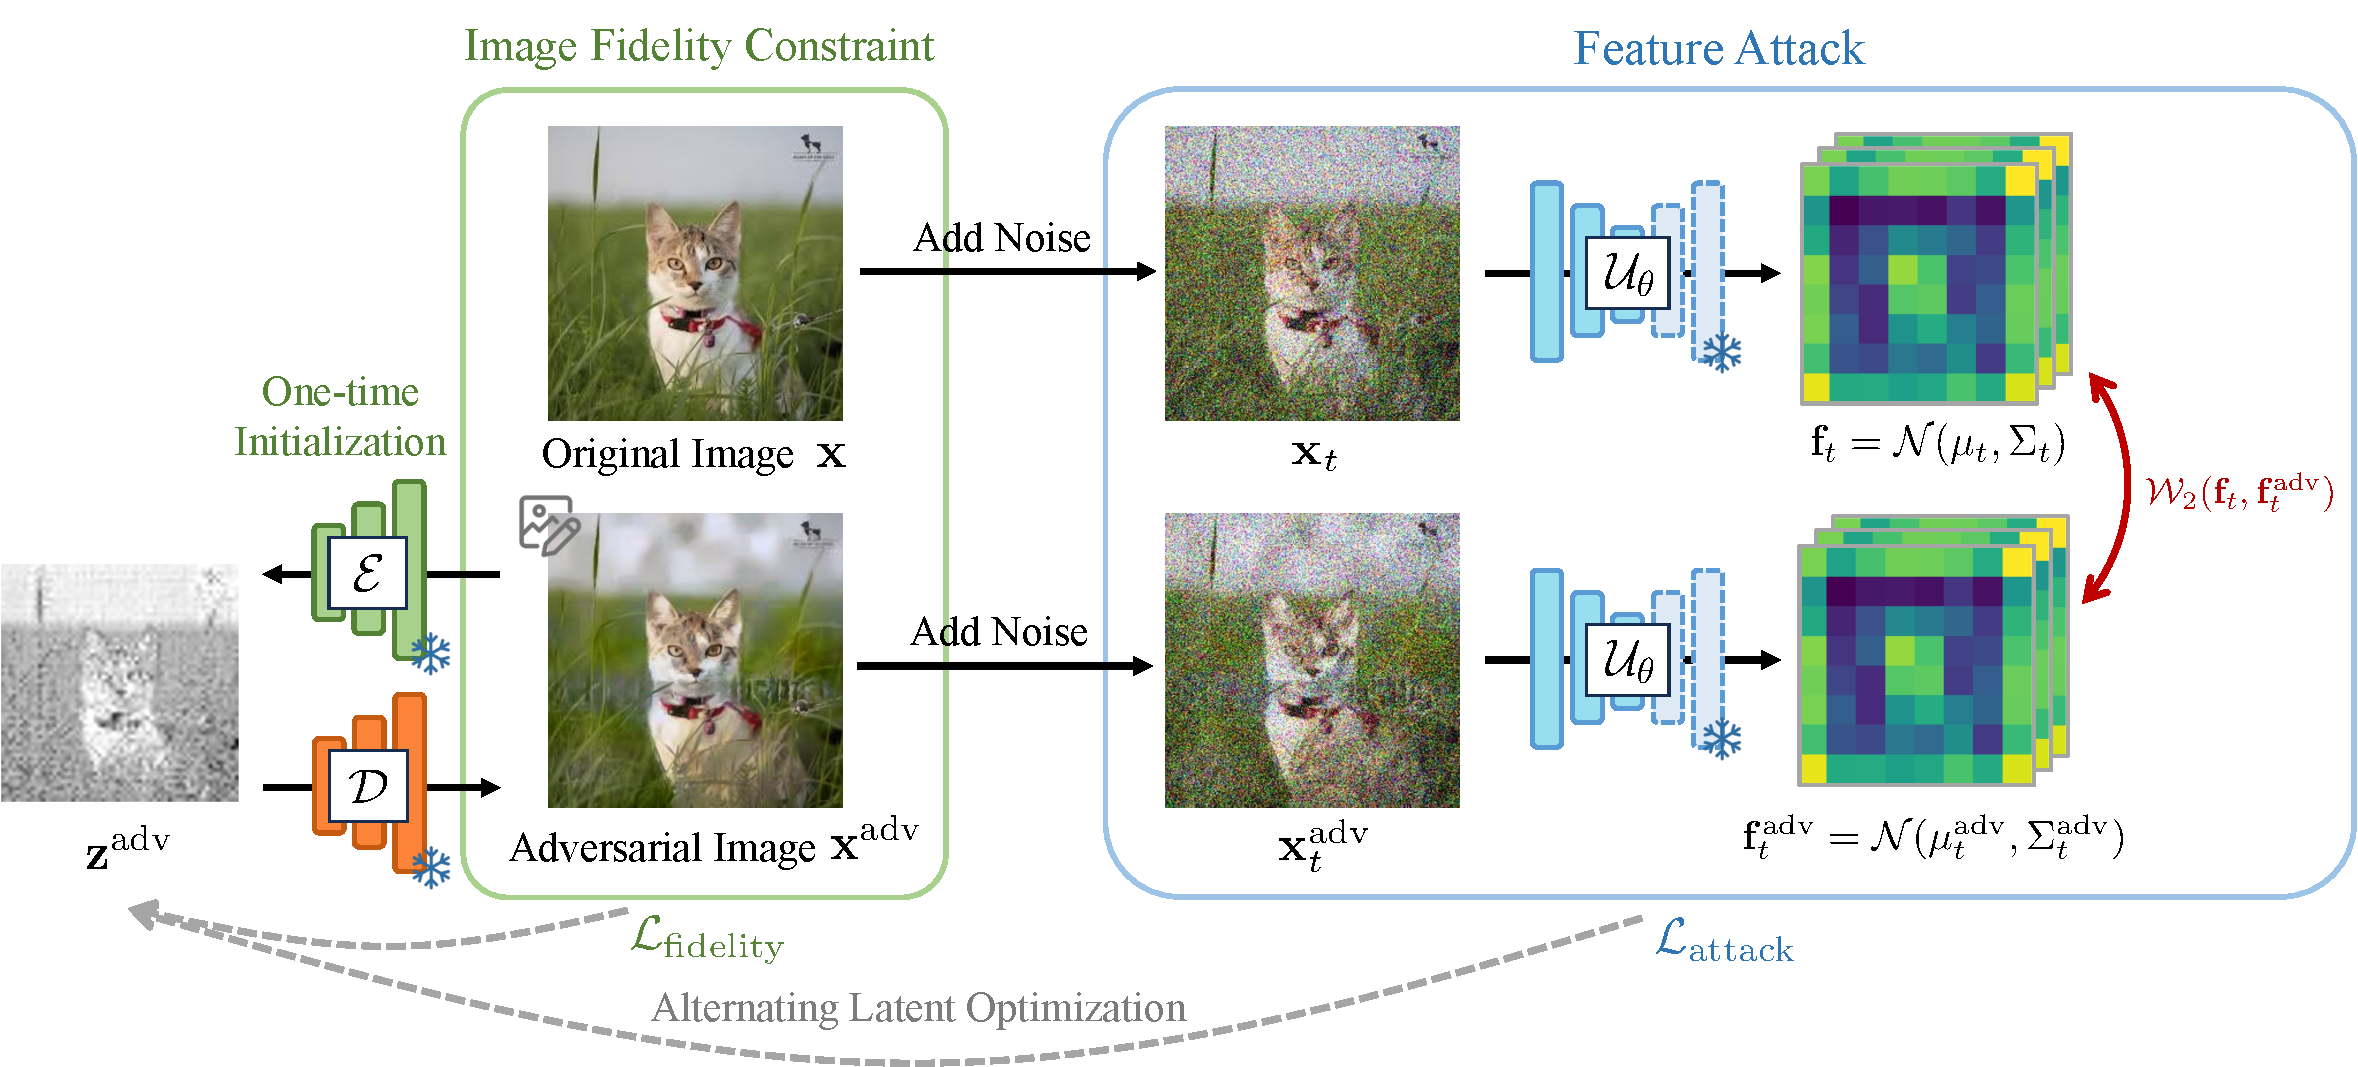
\includegraphics[width=1\linewidth]{figures/framework.pdf}
    \caption{Overview of our AtkPDM$^{+}$ algorithm: Starting from the leftmost latent of the initial adversarial image  $\mathbf{z}^{\adv}$, we first decode back to pixel-domain to perform forward diffusion with both $\mathbf{x}$ and $\mathbf{x}^{\adv}$ and feed them to frozen victim UNet. We then extract the feature representation in UNet to calculate our $\mathcal{L}_\text{attack}$, aiming to distract the recognition of image semantics. We also calculate our $\mathcal{L}_\text{fidelity}$ in pixel-domain to constrain the optimization. Finally, the $\mathbf{z}^{\adv}$ is being alternatively updated by loss gradients.}
    \label{framework}
\end{figure*}


\subsection{Overview}

To achieve effective protection against diffusion-based editing, we aim to push the protected sample away from the original clean sample by disrupting the intermediate step in the reverse diffusion process. For practical real-world applications, it's essential to ensure the protected image is perceptually similar to the original image. In practice, we uniformly sample the value of the forward diffusion step $t \sim [0, T]$ to generate noisy images and then perform optimization to craft the adversarial image $\mathbf{x}^{\adv}$ via our attacking and fidelity losses, repeating the same process $n$ times or until convergence. Figure \ref{concept} depicts these two push-and-pull criteria during different noise levels, the successful attack is reflected in the light orange line where the reverse sample moves far away from the normal edition of the image. More specifically, our method can be formulated as follows:

\begin{equation}
    \begin{aligned}
        & \max_{\mathbf{x}^{\adv} \in \mathcal{M}}
        \mathbb{E}_{
        t,
        \mathbf{x}_t| \mathbf{x}, \mathbf{x}_t^{\adv}| \mathbf{x}}
         \left[-\mathcal{L}_\text{attack}(\mathbf{x}_t, \mathbf{x}_t^{\adv})\right] \\
        & \text{subject to } \mathcal{L}_\text{fidelity}(\mathbf{x}, \mathbf{x}^{\adv}) \leq \delta,
    \end{aligned}
    \label{eq:probelm_setting_constraint}
\end{equation}

\noindent where $\delta$ denotes the attacking budget. The details of the attacking loss $\mathcal{L}_\text{attack}$ and the fidelity loss $\mathcal{L}_\text{fidelity}$ will be discussed in the following sections.


\subsubsection{Framework.}
Our framework is illustrated in Figure~\ref{framework}. We fix two identical victim UNets to extract feature representations of clean and protected samples for optimizing to push away from each other. A protection loss is jointly incorporated to constrain the optimization. After $N$ iterations, we segment out only the protecting main object of the image for better imperceptibility of image protection.

\subsection{Proposed Losses}
We propose two novel losses as optimization objectives to craft an adversarial example efficiently without running through all the diffusion steps. Attacking loss is designed to distract the feature representation in denoising UNet; Protection loss is a constraint to ensure the image quality. For notation simplicity, we first define the samples $\mathbf{x}, \mathbf{x}^{\adv}$ in different forwarded steps. 

Let $\mathcal{F}(\mathbf{x}, t, \epsilon) = \sqrt{\bar{\alpha}_t} \mathbf{x} + \sqrt{1-\bar{\alpha}_t} \epsilon$ be the diffusion forward process. Given timestep $t$ sample from $[0, T]$, noises $\epsilon_1, \epsilon_2$ sample from $\normaldist$. We denote $\mathbf{x}_t = \mathcal{F}(\mathbf{x}, t, \epsilon_1)$, and $\mathbf{x}^{\adv}_t = \mathcal{F}(\mathbf{x}^{\adv}, t, \epsilon_1)$.

\subsubsection{Attacking Loss.}
Our goal is to define effective criteria that could finally distract the reverse denoising process. PhotoGuard~\cite{salman2023raisingcostmaliciousaipowered} proposed to backpropagate through all the steps of the reverse denoising process via PGD, however, this approach is prohibitively expensive, Diff-Protect~\cite{xue2024effectiveprotectiondiffusionbased} proposed to avoid the massive cost by leveraging Score Distillation~\cite{poole2022dreamfusiontextto3dusing2d} in optimization. However, Diff-protect relies heavily on gradients of attacking encoder of an LDM as stated in their results. In PDM, we don't have such an encoder to attack; nevertheless, we find that the denoising UNet has a similar structure to encoder-decoder models, and some previous works~\cite{lin2024diffusionmodelperceptualloss, li2023fasterdiffusionrethinkingrole} characterize this property to accelerate and enhance the generation. From our observations of the feature roles in denoising UNets, we hypothesize that distracting specific inherent feature representation in UNet blocks could lead to effectively crafting an adversarial image. In practice, we first extract the feature representations of forwarded images $\mathbf{x}_t$ and $\mathbf{x}^{\adv}_t$ in frozen UNet blocks of timestep $t$. Then, we adopt 2-Wasserstein distance~\cite{arjovsky2017wasserstein} to measure the discrepancy in feature space. Note that we take the negative of the calculated distance, as we aim to pull the $\mathbf{x}^{\adv}_t$ away from $\mathbf{x}_t$. Formally, the attacking loss $\mathcal{L}_\text{attack}$ is defined as:
\begin{equation}
    \mathcal{L}_\text{attack}(\mathbf{x}_t, \mathbf{x}^{\adv}_t)
    =-\mathcal{W}_2 \left(
    \mathcal{U}^\text{(mid)}_{\theta}(\mathbf{x}_t), \mathcal{U}^\text{(mid)}_{\theta}(\mathbf{x}^{\adv}_t)
    \right).
\end{equation}

\noindent Assuming the feature distributions approximate Gaussian distributions expressed by mean $\mu_t$ and $\mu_t^{\adv}$, and non-singular covariance matrices $\Sigma_t$ and $\Sigma_t^{\adv}$. The calculation of the 2-Wasserstein distance between two normal distributions is viable through the closed-form solution~\cite{dowson1982frechet, olkin1982distance, chen2018optimal}:

\begin{equation}
    \begin{aligned}
        & \mathcal{W}_2^2(\mathcal{N}(\mu_t, \Sigma_t), \mathcal{N}(\mu_t^{\adv}, \Sigma_t^{\adv}))
        = \|\mu_t-\mu_t^{\adv}\|_2^2 \\
        & \qquad + \text{trace} (\Sigma_t + \Sigma_t^{\adv}
        -2({\Sigma_t^{\adv}}^{\frac{1}{2}}\Sigma_t{\Sigma_t^{\adv}}^{\frac{1}{2}})^\frac{1}{2} ).
    \end{aligned}
    \label{eq:wasserstein_distance}
\end{equation}

\subsubsection{Fidelity Loss.}
To control the attack budget for adversarial image quality, we design a constraint function that utilizes the feature extractor from a pretrained classifier for calculating fidelity loss. In our case, we sum up the 2-Wasserstein feature losses of $L$ different layers. Specifically, we define $\mathcal{L}_\text{fidelity}$ as:
\begin{equation}
    \mathcal{L}_\text{fidelity}(\mathbf{x}_t, \mathbf{x}^{\adv}_t)
    = \sum_{\ell=1}^L \mathcal{W}_2(\phi_\ell(\mathbf{x}), \phi_\ell(\mathbf{x}^{\adv})),
\end{equation}
where $\mathcal{W}_2$ denotes 2-Wasserstein distance and $\phi_\ell$ denotes layer $\ell$ of the feature extractor.


\subsection{Alternating Optimization for Adversarial Image}
We solve the constrained optimization problems via alternating optimization to craft the adversarial images, detailed optimization loop of AtkPDM$^{+}$ is provided in Algorithm ~\ref{alg:attdpmplus}. AtkPDM algorithm and the derivation of the alternating optimization are provided in Appendix.


\subsection{Latent Optimization via Pretrained-VAE}
Previous works suggest that diffusion models have a strong capability of resisting adversarial perturbations~\cite{xue2024pixelbarrierdiffusionmodels}, making them hard to attack via pixel-domain optimization. Moreover, they are even considered good purifiers of adversarial perturbations~\cite{nie2022diffusionmodelsadversarialpurification}. Here we propose a latent optimization strategy that crafts the ``perturbation'' in latent space. We adopt a pre-trained Variational Autoencoder (VAE) ~\cite{kingma2014autoencoding} to convert images to their latent space, and the gradients will be used to update the latent, after N iterations or losses converge, we decode back via decoder $\mathcal{D}$ to pixel domain as our final protected image. The motivation for adopting VAE is inspired by MPGD~\cite{he2024manifold}. This strategy is effective for crafting a robust adversarial image against pixel-domain diffusion models while also better preserving the protection quality rather than only incorporating fidelity constraints. The constraint optimization thereby becomes: 
\begin{equation}
\begin{aligned}
    & \max_{\mathbf{z}^{\adv}}
    \mathbb{E}_{
    t,
    \mathbf{x}_t| \mathbf{x}, \mathbf{x}_t^{\adv}| \mathcal{D}(\mathbf{z}^{\adv})}
    \left[-\mathcal{L}_\text{attack}(\mathbf{x}_t, \mathbf{x}_t^{\adv})\right] \\
    & \text{subject to } \mathcal{L}_\text{fidelity}(\mathbf{x}, \mathcal{D}(\mathbf{z}^{\adv})) \leq \delta.
\end{aligned}
\label{eq:probelm_setting_constraint}
\end{equation}

\noindent Detailed latent optimization loop is provided in Algorithm~\ref{alg:attdpmplus}.


\begin{algorithm}[t]
    \caption{AtkPDM$^{+}$}
    \label{alg:attdpmplus}
    \small{
    \begin{algorithmic}[1] 
        \STATE{\textbf{Input:}
        Image to be protected $\mathbf{x}$, attack budget $\delta > 0$, step size $\gamma_1, \gamma_2>0$, \textcolor{black}{VAE encoder $\mathcal{E}$, and VAE decoder $\mathcal{D}$}}
        \STATE{\textbf{Initialization:} $\mathbf{x}^{\adv} \leftarrow \mathbf{x}$, $L_\text{attack} \leftarrow \infty$}
        \STATE{\textcolor{black}{Encode adversarial image to latent space: $\mathbf{z}^{\adv} \leftarrow \mathcal{E}(\mathbf{x}^{\adv})$}}
        \WHILE{$L_\text{attack}$ not convergent}
            \STATE{\textcolor{black}{Decode adversarial latent to pixel space: $\mathbf{x}^{\adv} \leftarrow \mathcal{D}(\mathbf{z}^{\adv})$}}
            \STATE{Sample timestep: $t \sim [0, T]$}
            \STATE{Sample noise: $\epsilon_1, \epsilon_2 \sim \normaldist$}
            \STATE{Compute original noisy sample: $\mathbf{x}_t \leftarrow \mathcal{F}(\mathbf{x}, t, \epsilon_1)$}
            \STATE{Compute adversarial noisy sample: $\mathbf{x}^{\adv}_t \leftarrow \mathcal{F}(\mathbf{x}^{\adv}, t, \epsilon_2)$}
            \STATE{\textcolor{black}{Update $\mathbf{z}^{\adv}$ by Gradient Descent: \\
            $\mathbf{z}^{\adv} \leftarrow \mathbf{z}^{\adv} -
            \gamma_1 \sign(\nabla_{\mathbf{z}^{\adv}} \mathcal{L}_\text{attack}(\mathbf{x}_t, \mathbf{x}^{\adv}_t))$}}
            \WHILE{$\mathcal{L}_\text{fidelity}(\mathbf{x}, \textcolor{black}{\mathcal{D}(\mathbf{z}^{\adv})}) > \delta$}
            \STATE{ 
            \textcolor{black}{$\mathbf{z}^{\adv} \leftarrow \mathbf{z}^{\adv} -
            \gamma_2 \nabla_{\mathbf{z}^{\adv}} \mathcal{L}_\text{fidelity}(\mathbf{x}, \mathcal{D}(\mathbf{z}^{\adv}))$}}
            \ENDWHILE
        \ENDWHILE
        \STATE{\textcolor{black}{Decode adversarial latent to pixel space: $\mathbf{x}^{\adv} \leftarrow \mathcal{D}(\mathbf{z}^{\adv})$}}
        \RETURN {$\mathbf{x}^{\adv}$}
    \end{algorithmic}
    }
\end{algorithm}

